After the filtered odometry data and filtered GPS data are obtained, in this project the last step of the trajectory smoothing is to combine these two data sets together. The method used in this case is ISAM2 in \cite{5979641}.

The steps taken are similar to those in processing GPS data. It is noticeable that the odometry obtained from Figure \ref{fig:Gyrodometry} can be a good metric for orientation, as the details of filtered odometry are similar to those of the ground truth. In contrast, the absolution position of the filtered GPS data is similar to that of the ground truth. By tuning the covariance values($\sigma$) in linear and angular direction, the final filtered graph is shown in Figure \ref{fig:Final plot}.

\begin{figure}[hbt!]
    \centering
    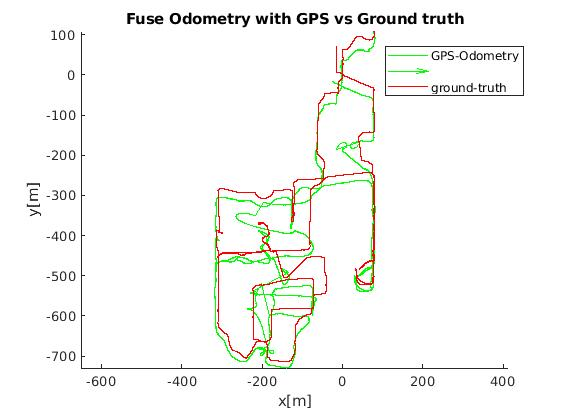
\includegraphics[width = 0.8\linewidth]{media/GPS+Odometry3.jpg}
    \caption{\textit{Compare filtered data with ground truth.}}
    \label{fig:Final plot}
\end{figure}